
% JuliaCon proceedings template
\documentclass{juliacon}
\setcounter{page}{1}

\begin{document}

% **************GENERATED FILE, DO NOT EDIT**************

\title{MedPipe3D.jl: GPU accelerated medical image segmentation framework}

\author[1, 2]{Jakub Mitura}
\author[2]{Beata E. Chrapko}
\author[2]{Oliwia Bachanek-Mitura}
\affil[1]{National Information Processing Institute}
\affil[2]{Medical University of Lublin}

\keywords{Julia, Computer Tomography, CUDA, Medical Image Segmentation}

\hypersetup{
pdftitle = {My JuliaCon proceeding},
pdfsubject = {JuliaCon 2022 Proceedings},
pdfauthor = {Jakub Mitura, Beata E. Chrapko, Oliwia Bachanek-Mitura},
pdfkeywords = {Julia, Computer Tomography, CUDA, Medical Image Segmentation},
}



\maketitle

\begin{abstract}
%% Text of abstract
Medical image segmentation is a rapidly developing field of computer vision, which requires knowledge in radiologic imaging, mathematics, and computer science. Multiple software packages have been designed to  assist researchers in the area; however, some of these tools are no longer  effective for some users due to the rapidly changing scientific environment. This is the case for Julia language users that require support for an interactive programming development style that is unpopular among traditional software tools. Another characteristic of modern programming for three-dimensional medical imaging data is GPU acceleration, improving algorithms' performance when working on objects that can be represented as large arrays, such as those in 3D medical imaging. This work presents new Julia language software tools designed to fulfill emerging needs. The tools include a GPU-accelerated medical image viewer with annotation possibility that is characterized by a convenient programming interface. The work then presents a CUDA-accelerated medical segmentation metrics tool that supplies state-of-the-art implementations of algorithms required for the quantification of similarity between algorithm outputs and gold standards. Lastly, the work presents a set of utility tools that connect the packages mentioned above using an HDF5 file system.

\keywords{CUDA,computer tomography,medical image segmentation  }
\end{abstract}


\section{Introduction}
One field of computer vision that  has an immediate influence on societal wellbeing is the automation of diagnoses based on medical imaging. Multiple algorithms, known as medical image segmentation algorithms, can be used to recognize and label pathological and physiological structures. As in any other field of computer vision, supervised, semisupervised, and nonsupervised methods can be distinguished. The forms can also be divided into automatic and semiautomatic ones; in the latter case, user input is required.

A typical workflow includes:
\begin{enumerate}
  \item visual inspection of  the data and exploration of the metadata
  \item feature engineering to represent the data most effectively in the chosen model
  \item selection of the model with consideration for possible assumptions that could be encoded within it as inductive bias
  \item selection of the segmentation metric and cost function.
  \item after evaluation and debugging, reconsideration of  design choices to improve the model's performance
  \item reiteration until the model's performance is satisfactory
\end{enumerate}

Multiple software tools are widely available for all of the steps above; to implement any model robustly and efficiently, however, the appropriate tools must be used for a given domain. This involves considerations of the size of single image files, performance constraints, the required devices' interoperability, and the package interface's language.

In 3D medical image segmentation, one common difficulty is the size of the images, which can frequently reach multiple gigabytes per patient. This demands parallelization to achieve good execution times. Currently, the most effective parallelization in medical imaging can be achieved using GPU architectures. Among tools used for medical segmentation metrics, the possibility of GPU acceleration is highly desirable. Such tools are available, for example, in MONAI \cite{MONAI} or TensorFlow \cite{tensorflow}; most have their interfaces written in the Python programming language. This is an advantage because it makes collaboration between data scientists easier. Python is the most popular data science language and is considered easy to use; however, it also leads to some specific issues, the most important of which is relatively low performance. Popular Python libraries usually solve this problem by having the main code written in a high-performance language like C++ and supplying a Python interface. Apart from the additional work necessary to write and maintain such libraries, they also encounter significant problems with the interoperability of Python packages. This is known as the 'two-language' problem. One of the best solutions to it is the Julia programming language \cite{Julia}. The Julia ecosystem contains multiple packages that support various aspects of GPU programming, including CUDA.jl \cite{besard2019prototyping} and ParallelStencil.jl \cite{ParallelStencil}, which can significantly simplify the development of GPU accelerated algorithms.

\section{Visual inspection}

\begin{figure}[t!]
	\centering
	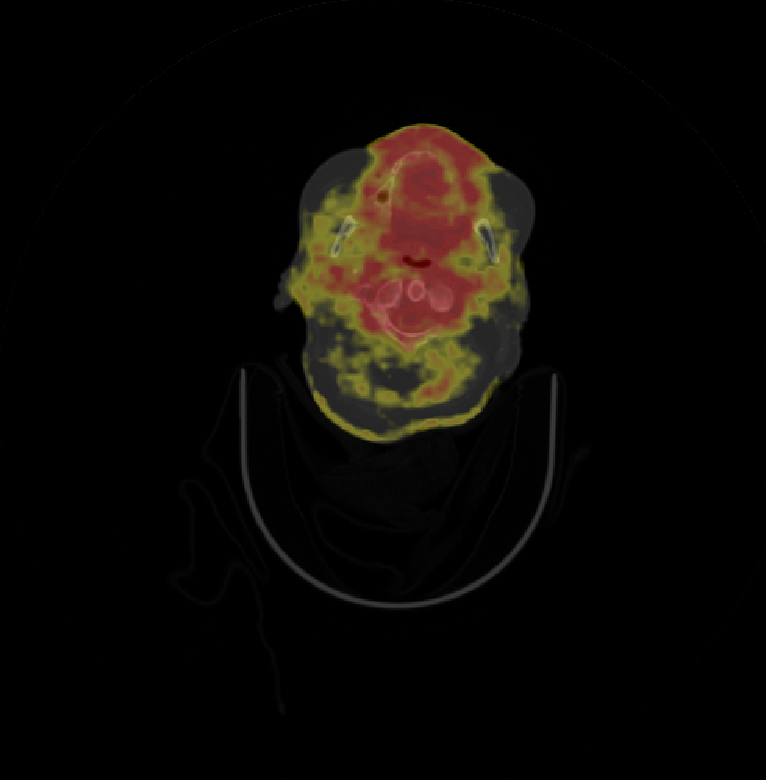
\includegraphics[width=0.5\textwidth]{PETCTCORONAL.png}
	\caption{Transverse display FDG PET/CT.}
	\label{fig:PETCTCORONAL}
	\centering
\end{figure}

The visual inspection of 3D data demands specialized software. Although multiple high-quality applications created for viewing and annotating are available, most require particular configurations and are not always convenient to use during the rapid development phase. In Julia, a typical workflow includes constant experimentation using the interactive environment, read--eval--print loop (REPL), which increases development efficiency. However, current 3D visualization tools are poorly suited to such a workflow. To address this issue, these authors have developed a new 3D visualization and annotation tool, MedEye3d \cite{Mitura2021}, characterized by high performance, low memory consumption, and an interface that is designed to be easily accessible from the REPL command line or keyboard shortcuts. The intended usage pattern includes no typical graphical user interface elements (such as buttons). This decreases the amount of screen space occupied by the application and makes it easier to use  as a separate window next to the chosen Julia integrated development environment (IDE). Despite this purposeful simplicity, all crucial functionalities required for displaying 3D medical imaging are easily accessible via keyboard shortcuts. In the case of the development of semiautomatic algorithms, annotations on the image are easy to perform, and the results are immediately available in the Julia REPL for further processing. Figure \ref{fig:PETCTCORONAL} shows an example of the display.

\section{Problem Statement and Research Objectives}
Although Julia is characterized by a plethora of excellent scientific software packages, to the best knowledge of the authors, it lacks some of the tools necessary for 3D medical segmentation. The biggest problems seem to be the lack of efficient visualization and evaluation tools. This work aims to provide the scientific community with those missing software solutions and, by doing so, to popularise a study on 3D medical segmentation in the Julia language community.


\section{Evaluation metrics}

Two primary considerations dictate the selection of evaluation metrics. The first is that the chosen metric quantifies the similarity between some gold standard and the algorithm's output. To assess this, some measure of domain knowledge related to the data on which the algorithm will be run is necessary. The second requirement is that the chosen metric function possesses  the properties required for optimization. In most cases, this means that the gradient of the metric can be defined so that it can be used, for example, in the backpropagation of the neural network. The second requirement leads, in some cases, to modifications of the metric function itself. The metric subjected to the optimization algorithm is called the cost function, and, by convention, small values should represent the large similarity between compared data. The first consideration is, arguably, more important from an algorithm design perspective, as a researcher must be specific that a reduction in the cost function value indeed leads to the increased similarity between the measured entities in a meaningful way. The cost functions traditionally defined for standard images are frequently unable to measure the similarity between the gold standard and the algorithm output in medical image segmentation. This problem is particularly evident in the case of three-dimensional data.

In medical segmentation, some of the most influential works that describe segmentation metrics are those published by Renard et al. \cite{Nature} and by Taha et al. \cite{TahaMainSegm}. Those works stressed that optimal metrics might differ depending on the problem. For example, in multiple cases, a large interclass discrepancy exists concerning its representation in the data; for this reason, one of the most commonly used segmentation metrics is Dice. In the work of Taha et al. \cite{TahaMainSegm}, multiple algorithms, including the Dice metric, are implemented using a confusion matrix (which includes several true positive, false positive, true negative, and false negative entries). This group of algorithms opens new opportunities to use multiple metrics simultaneously without incurring significant performance penalties and to validate using other criteria, such as visual inspection. Frequently, not only the number of voxels that are correctly or incorrectly labeled is essential, but also their spatial distribution. In this case, distance metrics like Mahalanobis or Hausdorff distance should be considered. Algorithms that consider distance are typically far more computationally intensive.

Two main frameworks dominate the subfield of machine learning in medical imaging segmentation metrics: Pymia \cite{Pymia} and MONAI \cite{MONAI}. In both cases, the user interface is written in Python. MONAI \cite{MONAI} implements multiple  highly-optimized metrics that are particularly prevalent in neural networks with available Compute Unified Device Architecture (CUDA) acceleration; yet, it lacks most of those described in \cite{TahaMainSegm}. MONAI is  based on PyTorch \cite{pytorch}. Pymia \cite{Pymia} implements all of the algorithms described in \cite{TahaMainSegm} and is framework independent, but lacks GPU acceleration, which may drastically limit its performance in cases of large data objects and such cases are highly common in modern medical imaging. In order to remedy this situation authors published the MedEval3d \cite{medEval}, with implementations of multiple image segmentation metrics with CUDA acceleration.


\section{Data management}
Medical imaging data in clinical settings is usually stored in the Digital Imaging and Communications in Medicine (DICOM) \cite{dicom} standard. Apart from keeping the data representing a given variable in each voxel of a study, DICOM can hold rich metadata, such as patients' names and ages, and details about the acquisition technique.  The standard was primarily designed for optimizing the display and storage of data and not its processing; thus, operations like partial loading or data queries lack efficiency.

Hierarchical Data Format HDF5 \cite{hdf5} originates from a high-performance computing ecosystem. It is recognized as an efficient and convenient data format for storing and processing medical imaging data \cite{hdf5Medical}. Apart from its high performance, the format is characterized by its ability to save and process multidimensional data and its optimization for large multidimensional arrays. This characteristic is uncommon, as most traditional data formats are optimized for tabular data and store image data in binary object data types (BLOB), with a limitation that no queries can be performed for data in a BLOB. HDF5, contrarily, makes queries and partial loading of stored multidimensional arrays. As with other popular data formats, it has programming APIs in multiple widely-used languages, such as Python, C++, and Julia.

The HDF5 data format seems optimal for processing 3D medical imaging, as it has excellent support for multidimensional data, supports the saving of the metadata of those arrays (like the DICOM format), and has good query performance and convenient programming interfaces (like traditional database formats). Another unique feature is the possibility of direct data loading from persistent storage to GPU global memory without intermediate storage in a CPU's RAM  \cite{hdf5GPU}; this feature, however, will not be used in this work for the sake of simplicity.

\subsection{Experiments}
\subsubsection{Evaluation metrics}
All experiments were conducted on a Windows PC (Intel Core I9 10th gen., GeforceRTX 3080), using data from the CT-ORG \cite{CTORG} dataset on images of size ($512 \times 512 \times 826$). The time needed to calculate the metrics was estimated in the case of the Julia code using BenchamrkTools.jl \cite{BenchmarkTools}. For testing the Python libraries, an internal python module, timeit, was used. The results of the experiments mentioned above are summarised in Figure \ref{fig:bk}. In all cases, the data was already stored in RAM for CPU computations, or in GPU memory for CUDA computations; for this reason, memory transfer times were not included.

\begin{figure}[h!]
	\centering
	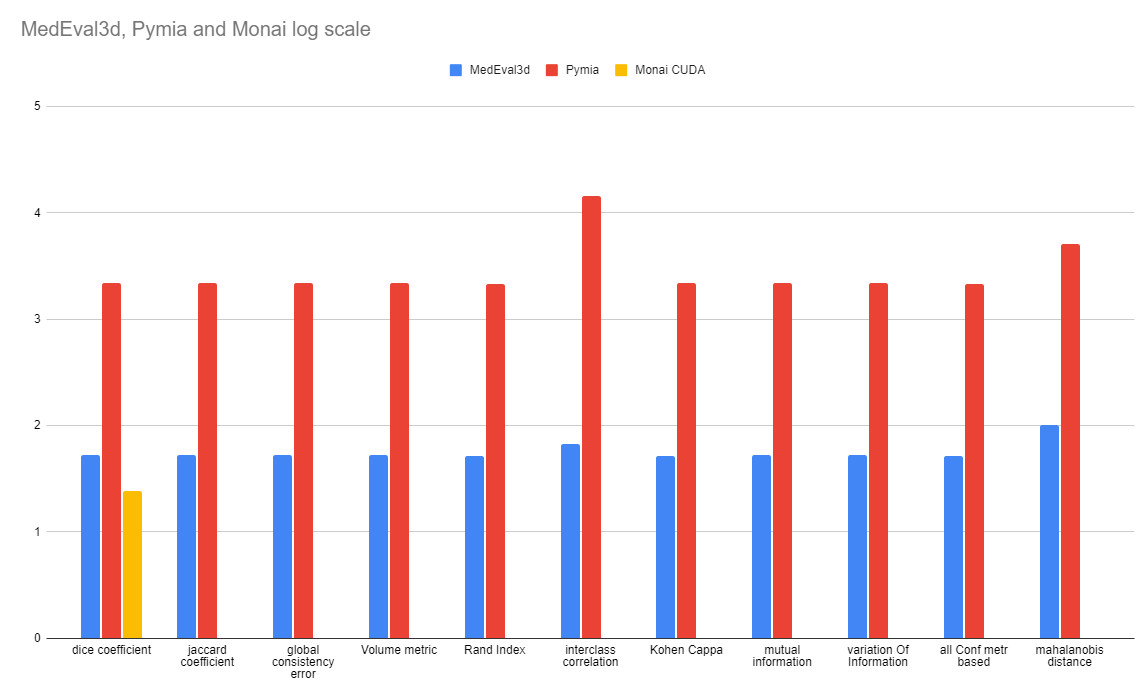
\includegraphics[width=\columnwidth]{bk.png}
	\caption{Comparison of median times needed to calculate given metrics in log scale. For MONAI, only the CUDA-accelerated algorithm was considered. The dimensionality of the data was ($ 512x512x826 $).  }
	\label{fig:bk}
\end{figure}

\subsubsection{Visualisation}

To measure the time necessary to  render the image on the GPU, synchronization was performed using the OpenGL glFinish() function.
Cross-section plane translation changes the single coordinate that specifies the plane in a chosen cross-section. The time needed to accomplish this is measured as the number of milliseconds between rendering the commands using BenchamrkTools.jl \cite{BenchmarkTools}. 

Response to the left click time of the mouse was measured as the difference between the time reported in the callback registered to the GLFW window and the end of the execution of a command designed to render the visible change on the chosen texture.

\begin{figure}[t!]
	\centering
	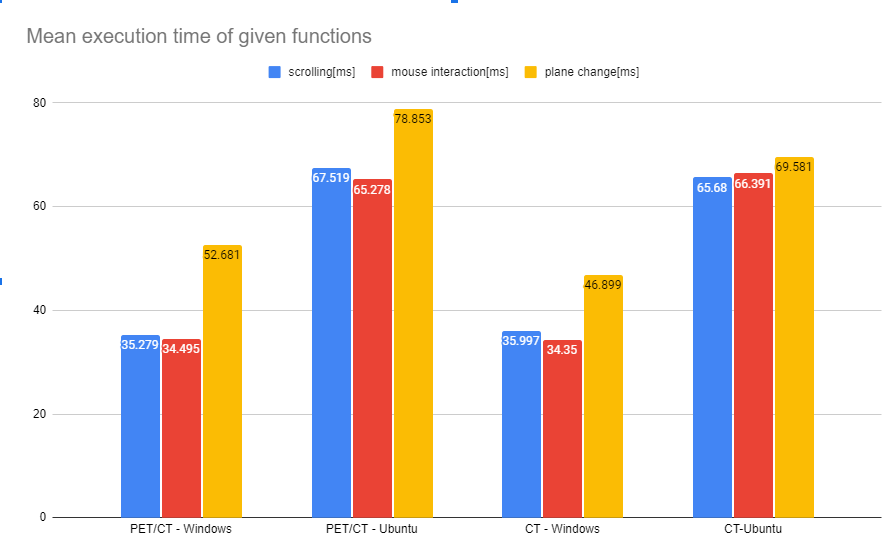
\includegraphics[width=\columnwidth]{Przechwytywanie.png}
	\caption{Execution times depending on function and machine used.}
	\label{fig:Przechwytywanie}
	\centering
\end{figure}

The time required for a cross-section plane change (for example, from transverse to sagittal) was defined as the difference in time between the invocation of a GLFW callback (which itself is invoked by the appropriate user interaction) and the end of the rendering function execution.
The results of the experiments are summarised in Figure \ref{fig:Przechwytywanie}. It is visible that the time required to complete functions in the case of the Ubuntu laptop was longer; yet, considering its far inferior hardware, this was to be expected. The reduced performance did not affect the user experience.


Memory use was tested using actual data from PET/CT. The data uploaded to the display constituted three matrices of Float32, UInt8,  and Int16 data types, as well as a 2000x8000 matrix that holds text data. 
In the case of the Windows 10 system, dedicated GPU memory use was evaluated using the Details section of the Task Manager and oscillated between 38 and 39.5 MB. In the case of the Ubuntu laptop, Nvidia System Monitor was used to estimate GPU memory usage, and dedicated GPU memory usage oscillated around 21MB. 

\section{Conclusions}
Medical image segmentation is a complex task that requires knowledge from medicine, engineering, and mathematics. Multiple software tools have been developed to make the task of developing such algorithms as manageable as possible. However, the need for further specialization of these tools has emerged due to rapid advancements in machine learning and medical imaging. Although most of the research community's needs may be met by existing solutions, there are use cases in which current solutions are inadequate. One example of such a case is Julia's programming language ecosystem. 
Researchers who wish to work in the Julia programming language due to its rich ecosystem of scientific libraries or its high performance, both in terms of execution time and development time. One requirement of developing medical segmentation algorithms in Julia is that all necessary steps be completed using Julia with the possible exception of preprocessing, which often must be performed only once.

The programming framework presented in this work is a response to the changing software environment and is implemented in an emerging programming language, Julia. It also uses GPU acceleration, which delivers vast performance improvements over CPU-based algorithms, and uses modern programming approaches like reactive functional style in GUI programming. Critically for convenient rapid prototyping, all of the programming processes can be performed with the help of Julia REPL. To the best knowledge of the authors, multiple metrics implemented in the presented software are characterized by the shortest execution times not only in Julia but also in all popular open source solutions. 

To make the development process even easier, the final section of this work presents an additional set of utility functions, which, for example, add a persistence layer  using the HDF5 system. All the tools offered in this work are highly composable and may be used in isolation, which constitutes another crucial advantage. 

\section{Acknowledgement}
The package is open source and available on GitHub at: https://github.com/jakubMitura14/MedPipe3D.jl under the Apache license. In case of feature requests, bug reporting, or contribution proposals, don't hesitate to contact the corresponding author via LinkedIn: https://linkedin.com/in/jakub-mitura-7b2013151/ or in the issues section of the GitHub repository.

% **************GENERATED FILE, DO NOT EDIT**************

\bibliographystyle{juliacon}
\bibliography{ref.bib}


\end{document}

% Inspired by the International Journal of Computer Applications template
